\documentclass[12pt]{extbook}

% \usepackage[paperwidth=5.5in, paperheight=8.5in, margin=0.3in]{geometry}
% \usepackage[paperwidth=8.5in, paperheight=11in, margin=0.5in]{geometry}

\usepackage[paperwidth=5.5in, paperheight=8.5in,bindingoffset=0.125in,margin=0.8in]{geometry}

% Fonts and typography

%% Typography
\usepackage[no-math]{fontspec}
\defaultfontfeatures{Mapping = tex-text, Scale = MatchLowercase}

\usepackage{csquotes}

%% Fonts
\setmainfont{Adobe Garamond Pro}
\setsansfont{Adobe Garamond Pro}
\setmonofont[Mapping=tex-ansi]{Menlo}

\newfontfamily\coder[Mapping=tex-ansi]{Menlo}

%% Set Sans font in headings
% \usepackage{sectsty}
% \allsectionsfont{\sffamily}

%% Set polyglossia language
\usepackage{polyglossia}
\setdefaultlanguage{english}

% \usepackage[fontsize=16pt]{scrextend}

\usepackage{titlesec}
% \titleformat{\chapter}[display]
%   {\normalfont\sffamily\huge\bfseries\centering}
%   {\chaptertitlename\ \thechapter}{20pt}{\Huge}
\titleformat{\section}
  {\normalfont\sffamily\huge\bfseries\centering}
  {\thesection}{1em}{\Huge}
% \titlespacing*{\chapter}{0pt}{30pt}{20pt}

% \usepackage{titlesec}
% \titleformat{\chapter}[display]
% {\normalfont\huge\bfseries}{\centering\chaptertitlename\ \thechapter}{20pt}{\Huge}


% new page for every chapter
% \newcommand{\sectionbreak}{\clearpage}

% Page

%% Use full page in book style
% \usepackage{fullpage}

\usepackage{fancyhdr}
\pagestyle{fancy}
\fancyhf{}
\fancyhead{}
\fancyfoot{}
\renewcommand{\headrulewidth}{0.1pt}
% \headrulewidth 0.0pt
% \fancyfoot[C]{\thepage}
\fancyfoot[RO, LE] {\thepage}

%% Set line spacing
\usepackage{setspace}
\setstretch{1.2}

%% Disable paragraph indentation
\usepackage{parskip}

\usepackage{afterpage}

\newcommand\blankpage{%
    \null
    \thispagestyle{empty}%
    \addtocounter{page}{-1}%
    \newpage}


%% Start sections from new page
% \let\stdsection\section
% \renewcommand\section{\newpage\stdsection}

\usepackage[labelformat=empty]{caption}

% Images
\usepackage{graphicx}

\usepackage{pdfpages}


\usepackage{xcolor}

%% Tango color scheme
\definecolor{SkyBlue}{HTML}{3465A4}
\definecolor{DarkSkyBlue}{HTML}{204A87}

\definecolor{Plum}{HTML}{75507B}

\definecolor{ScarletRed}{HTML}{CC0000}

\definecolor{Aluminium1}{HTML}{EEEEEC}
\definecolor{Aluminium6}{HTML}{2e3436}

\definecolor{Black}{HTML}{000000}

\definecolor{Grayr}{HTML}{777777}


\usepackage{listings}

\lstdefinelanguage{CODER}{%
  morekeywords = {PAU, JLS, OUIMTQ, ZSMELC, LP, ELJT, L, OLE, ELC, ZRS, XRSP, IRRETUJQ, IRRE, VLXPLMTQ, LTE, XMSLPUQ},
  ndkeywords = {class, export, boolean, throw, implements, import, this},
  % ndkeywordstyle = \color{Aluminium6}\bfseries,
  % identifierstyle = \color{Black},
  sensitive = false,
  comment = [l]{//},
  morecomment = [s]{/*}{*/},
  % commentstyle = \color{Plum}\ttfamily,
  stringstyle = \color{ScarletRed}\ttfamily,
  morestring = [b]',
  morestring = [b]"
}

\lstset{
  language = CODER,
  % backgroundcolor = \color{Aluminium1},
  extendedchars = true,
  basicstyle = \normalsize\ttfamily,
  showstringspaces = false,
  showspaces = false,
  tabsize = 1,
  breaklines = true,
  keywordstyle=\color{Grayr},
  showtabs = false
}

%% Normal enumerates processing
% \usepackage{enumerate}

%% Disable section numbers
% \setcounter{secnumdepth}{0}

\renewcommand\thesection{\arabic{section}}

\begin{document}

  % Title page
  % \thispagestyle{empty}
  % \pagestyle{myheadings}
  % \vspace*{\fill}
  %   \begin{center}
  %     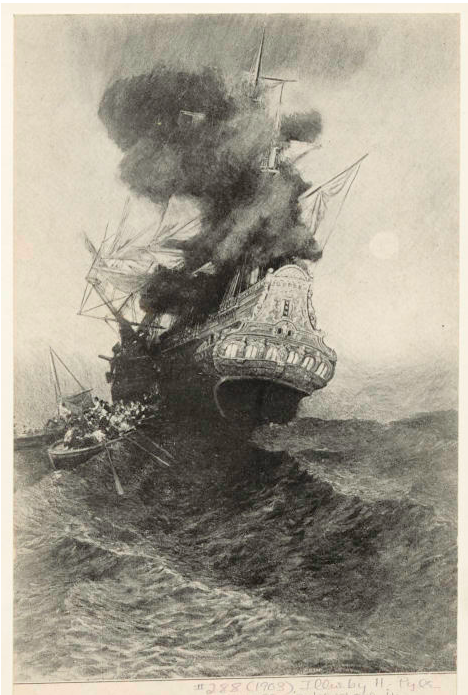
\includegraphics[width=0.98\textwidth]{img/title}
  %   \end{center}
  % \vspace*{\fill}

  % \begin{figure}
  % \noindent\makebox[\textwidth][c]{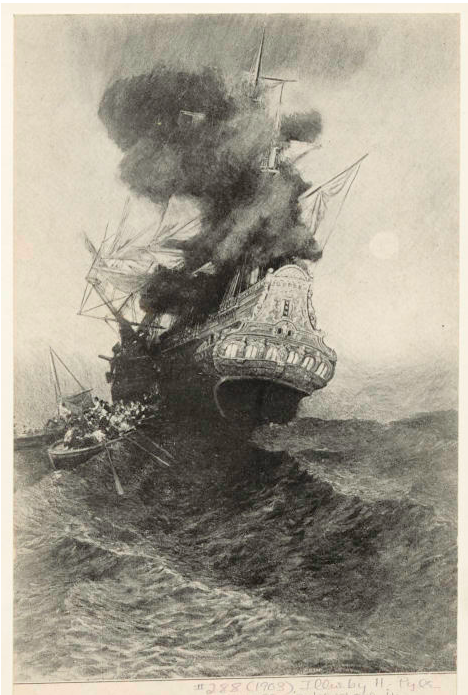
\includegraphics[width=1.4\textwidth]{img/title}}%
  % \end{figure}

  % \includepdf[pages={1}]{img/captain_z_title_2.pdf}

  \pagestyle{empty}
  \vspace*{\fill}
  \begin{center}
  \huge{Captain Z and the Treasure of Castle Island}\\[0.5cm]
  \end{center}
  \vspace*{\fill}
  % \afterpage{\blankpage}
  % \clearpage

  \begin{titlepage}
    \vspace*{\fill}
    \begin{center}
      \huge{Captain Z and the Treasure of Castle Island}\\[0.5cm]
      \large {Jimmy Vallandingham}\\[0.4cm]
    \end{center}
    \vspace*{\fill}
  % \clearpage
  \end{titlepage}
  
  \begingroup
  \footnotesize
  \parindent 0pt
  \parskip \baselineskip
  \vfill
  Captain Z and the Treasure of Castle Island \\
  Jimmy Vallandingham \\


  Copyright \textcopyright{} 2014 by Jimmy Vallandingham \\
  
  All rights reserved. No part of this publication may be reproduced, stored in a retrieval system, or transmitted in any form or by any means without prior written permission of the copyright owners. 
  
  If you want permission, just let me know.\\
  Contact information can be found at vallandingham.me


  ISBN: 978-1501048449

  First edition: October 2014

  \vfill
  vallandingham.me\\
  captainZbook.com
  \vspace*{2\baselineskip}
  \clearpage
  \endgroup

  \begingroup
  \vspace*{\fill}
  \begin{center}
  To my wife, daughter, and son.
  \end{center}
  \vspace*{\fill}
  \afterpage{\blankpage}
  \endgroup
  \setcounter{page}{0}
  \clearpage
  

  % \frontmatter
  
  \pagestyle{fancy}

  % Book contents
  $body$

\end{document}

